\documentclass[tikz,border=10pt]{standalone}
\usetikzlibrary{angles}

\begin{document}
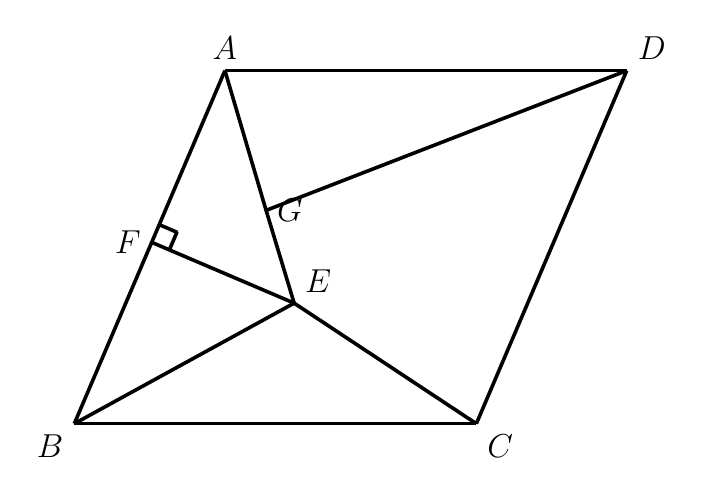
\begin{tikzpicture}[line width=1.3pt, line join=round]
\coordinate (A) at (-1.611,2.257);
\coordinate (B) at (-3.524,-2.227);
\coordinate (C) at (1.582,-2.227);
\coordinate (D) at (3.492,2.257);
\coordinate (E) at (-0.732,-0.696);
\coordinate (F) at (-2.541,0.076);
\coordinate (G) at (-1.088,0.482);



  
  \draw (A) -- (D);
  \draw (C) -- (D);
  \draw (B) -- (C);
  
  \draw (A) -- (F) -- (B);

  
  \draw (A) -- (G) -- (E);
  \draw (D) -- (G);

  \draw (B) -- (E);
  \draw (C) -- (E);
  \draw (E) -- (F);

  
  \draw pic[draw, angle radius=0.244cm] {right angle=A--F--E};

  
  \node[above] at (A) {\fontsize{13}{15.6}\selectfont $A$};
  \node[above right] at (D) {\fontsize{13}{15.6}\selectfont $D$};
  \node[below left] at (B) {\fontsize{13}{15.6}\selectfont $B$};
  \node[below right] at (C) {\fontsize{13}{15.6}\selectfont $C$};
  \node[above right] at (E) {\fontsize{13}{15.6}\selectfont $E$};
  \node[right] at (G) {\fontsize{13}{15.6}\selectfont $G$};
  \node[left] at (F) {\fontsize{13}{15.6}\selectfont $F$};
\end{tikzpicture}
\end{document}